\section{Theorie}
\label{sec:Theorie}
Licht kann als elektromagnetisch Welle verstanden werden.
Dringt eine Lichtwelle in durchsichtige Materie ein, so wechsel wirkt diese mit dem E-Feld der Elektronen.
Daraus resultiert eine Geschwindigkeitsänderung.
Die Geschwindigkeit des Lichts ist, aufgrund dieses Vorgangs, im Medium geringer als die Vakuum-Lichtgeschwindigkeit.
Licht, welches schräg von einem Medium ins andere übergeht, erfährt an der Grenzfläche durch den beschriebenen Vorgang eine Richtungsänderung.
Dieses Phänomen wird als Brechung bezeichnet.
Der Brechungsindex $n$ ist als das Verhältniss der beiden Geschwindigkeiten definiert:
\begin{equation}
  n= \frac{c_1}{c_2} .
\end{equation}
Die Lichtgeschwindigkeit im Medium ist auch von der Frequenz abhängig.
Der Brechungsindex ist demnach auch von der Frequenz des Lichts beziehungsweise der Wellenlänge $\lambda$ abhängig.
Diese Abhängigkeit wird Dispersion gennant.
In diesem Experiment ist die Dispersionskurve
\begin{equation}
  n= f(\lambda)
\end{equation}
von Interesse.
\subsection{Erklärung der Brechung nach dem Huygenschen Prinzip}
Licht erfährt bei dem Übergang in ein optisch dichteres oder dünneres Medium eine Richtungsänderung, diese kann durch Winkel ausgedrückt werden.
Trifft ein Lichtstrahl unter dem Winkel $\alpha$ auf eine Grenzfläche erfährt dieser eine Richtungsänderung und breitet sich unter dem Winkel $\beta$ in dem neuen Medium aus.
Nach dem Huygenschen Prinzip kann jeder Punkt einer bestehenden Wellenfläche als Zentrum einer kugelförmigen Elementarwelle verstanden werden.
Aus der Einhüllenden der Elemntarwellen bildet sich dann die neue Wellenfront.
Berücksichtigt man die erwähnten Winkelabhängigkeiten, dann kann der Brechungsindex in der Form
\begin{equation}
  \label{eq:snell}
  n = \frac{\sin(\alpha)}{\sin(\beta)}
\end{equation}
hergeleitet werden.
Die Gleichung \eqref{eq:snell} wird als Snellius-Brechungsgesetz bezeichnet.
\subsection{Ableitung der Disspersionsgleichung}
Nach Maxwells Theorie kann die Feldstärke einer Elektromagnetischen Welle durch
\begin{equation}
  E = E_0 \exp(i\omega t)
\end{equation}
beschrieben werden.
Damit lässt sich folgende Differentialgleichung der Bewegung formulieren:
\begin{equation}
  m_h \frac{d^2 x_h}{dt^2} +f_h \frac{d x_h}{dt} + a_h x_h = q_h E_0 \exp(i\omega t)  .
\end{equation}
Die Differentialgleichung kann umgeschrieben werden indem $x_h$ durch die Polarisation ersetzt wird:
\begin{equation}
  \label{eq:schwing}
  \frac{d^2 P_h}{dt^2} +\frac{f_h}{m_h} \frac{d P_h}{dt} + \frac{a_h}{m_h} P_h = \frac{N_q q_h^2}{m_h} E_0 \exp(i\omega t)  .
\end{equation}
Die Gleichung\eqref{eq:schwing} ist die Differentialgleichung einer erzwungenen Schwingung.
Diese hat die Lösung
\begin{equation}
  P_h =\frac{1}{\omega_h ^2 -\omega ^2 + i\frac{f_h}{m_h}\omega}\frac{N_q q_h^2}{m_h} E_0 \exp(i\omega t) .
\end{equation}
Die Gesamte Polarisation beträgt
\begin{equation}
  \label{eq:pol}
  P=\sum_{h} \frac{1}{\omega_h ^2 -\omega ^2 + i\frac{f_h}{m_h}\omega}\frac{N_q q_h^2}{m_h} E_0 \exp(i\omega t) .
\end{equation}
Die Polarisation ist gleich der dielektrischen Verschiebung in Materie vermindert um die dielektrische Verschiebung im Vakkum.
Damit kann Gleichung\eqref{eq:pol} umgeschrieben werden zu
\begin{equation}
  (\tilde{\varepsilon} -1)\varepsilon_0 = \sum_{h} \frac{1}{\omega_h ^2 -\omega ^2 + i\frac{f_h}{m_h}\omega}\frac{N_q q_h^2}{m_h} .
\end{equation}
Durch die abgeleitete Maxwellsche Relation
\begin{equation}
  \tilde{n}=\varepsilon
\end{equation}
kann der Zusammenhang zwischen Brechungsindex und Lichtfrequenz hergestellt werden.
Es folgt:
\begin{equation}
  \label{eq:n}
  \tilde{n} =  1 + \sum_{h} \frac{1}{\omega_h ^2 -\omega ^2 + i\frac{f_h}{m_h}\omega}\frac{N_q q_h^2}{m_h \varepsilon_0} .
\end{equation}
Dabei ist $\tilde{n}$ eine komplexe Größe der Form
\begin{equation}
  \tilde{n} = n(1 - ik) ,
\end{equation}
wobei $k$ die Absorbationskonstante von Licht in Materie darstellt.
Der Verlauf der Dispersionskurve wird für
\begin{equation}
  n^2 k \approx 0
\end{equation}
betrachtet.
Die Gleichung\eqref{eq:n} geht dann über in
\begin{equation}
  n^2 (\omega) = 1 + \sum_{h} \frac{N_h q_h ^2}{\varepsilon_0 m_h}\frac {1}{\omega ^2 -\omega_h ^2} .
\end{equation}
Aufgrund der Messbarkeit wird $\omega$ durch $\lambda$ ersetzt.
Damit folgt:
\begin{equation}
  n^2 (\lambda) = 1 + \sum_{h} \frac{N_h q_h ^2}{4 \pi^2 c^2 \varepsilon_0 m_h}\frac{\lambda^2\lambda_h ^2}{\lambda^2 - \lambda_h ^2} .
\end{equation}
Wenn die Betrachtete Materie nur die Absorptionsstelle $\lambda_1$ aufweist,

\noindent dann gilt für $\lambda << \lambda_1$
\begin{equation}
  \label{eq:a}
  n(\lambda) = 1 + \frac{N_1 q_1 ^2 \lambda_1 ^2}{4 \pi^2 c^2 \varepsilon_0 m_1}(1 + (\frac{\lambda_1}{\lambda})^2 + (\frac{\lambda_1}{\lambda})^4 + ...)
\end{equation}
und für $\lambda >> \lambda_1$
\begin{equation}
  \label{eq:b}
  n(\lambda) = 1 - \frac{N_1 q_1 ^2 }{4 \pi^2 c^2 \varepsilon_0 m_1}(\lambda^2+ \frac{\lambda^4}{\lambda_1 ^2} + \frac{\lambda^6}{\lambda_1 ^4} + ...)  .
\end{equation}
Damit entstehen die beiden Dispersionskurven in Abbildung \ref{fig:disp}.
\begin{figure}[H]
  \centering
  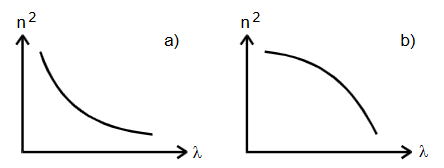
\includegraphics[scale=0.6]{content/disp.png}
  \caption{Gestalt der Dispersionskurven a) nach Gleichung\eqref{eq:a} und b) nach Gleichung\eqref{eq:b}\cite{v402}.}
  \label{fig:disp}
\end{figure}
\noindent Die dargestellten Kurven beschreiben die normale Dispersion.
Nimmt $n$ mit wachsender Wellenlänge $\lambda$ zu, dann liegt abnormale Dispersion vor.
